\documentclass{mgggarticle}
\usepackage[utf8]{inputenc}
\usepackage{amsmath}
\usepackage{parskip}
\usepackage{mathtools}
\usepackage{caption}
\usepackage{hyperref}
\usepackage{subcaption}


\usepackage{amsthm}
\newtheorem{Lemma}{Lemma}

\title{Discussion of Locality Splitting Measures}
\author{\name{Splittings Group}\affil{Voting Rights Data Institute 2019}}
\date{August 2019}

\DeclareMathOperator{\pop}{pop}
\DeclareMathOperator{\dis}{districts}
\DeclareMathOperator{\cou}{counties}


\version{1.0}

\titlespacing\section{0pt}{12pt plus 4pt minus 2pt}{0pt plus 2pt minus 2pt}
\titlespacing\subsection{0pt}{12pt plus 4pt minus 2pt}{0pt plus 2pt minus 2pt}
\titlespacing\subsubsection{0pt}{12pt plus 4pt minus 2pt}{0pt plus 2pt minus 2pt}

\begin{document}




\maketitle



\section*{Contributors}
{Taissa Gladkova, Ari Goldbloom-Helzner, Muniba Khan, Brandon Kolstoe, Jasmine Noory, Zachary Schutzman, Eric Stucky, \and Thomas Weighill} contributed to the research, analysis, coding, and writing of this report.


\vspace*{-1em}
	
\section*{About}
This report is the product of the Week 3 project on `splitting' at the 2019 Voting Rights Data Institute.  Our goal was to investigate ways to operationalize the general concept of `districts ought not to split political subunits'.  We considered legal and philosophical frameworks motivating this imperative, existing measures, and work done at the 2018 Voting Rights Data Institute.  Informed by this, we introduce a novel splitting measure which we call `naked boundary', which captures the extent to which the district lines fail to follow locality boundaries.


The code to compute these scores is now integrated into \texttt{gerrychain}.  Documentation for using these scores to evaluate your own plans or ensembles of plans can be found in the \texttt{gerrychain} documentation at \href{https://gerrychain.readthedocs.io}{\texttt{gerrychain.readthedocs.io}}.  The source code can be found in the \href{https://github.com/mggg/GerryChain/blob/master/gerrychain/updaters/locality_split_scores.py}{ \texttt{gerrychain} repository on GitHub}.

\tableofcontents




\section{Why shouldn't districts split localities?}
The reasons why one may want districts to keep localities whole are varied. The relevance of each of these motivations may vary from state to state -- for example, a state where counties play a large role in governing may consider the ``nested government'' argument to be stronger. We list here a non-exhaustive list of reasons which one may want to consider. We focus on the case of counties as that was the primary motivating example of a locality considered during the project's run.

\begin{enumerate}
\item \textbf{Existing law} -- nineteen out of fifty states require or advise for their congressional districts to follow political boundaries. Of the twelve that get into any specifics, all twelve specifically mention counties.

\item \textbf{Limiting gerrymandering} -- it is possible that restricting the ability of districts to split up larger units such as counties may limit the ability of map-drawers to gerrymander.  There is some evidence based on ensembles for this in the \emph{Virginia criteria paper}. As further informal evidence for this fact, consider the following map of NC. The underlying choropleth shows the vote share from the 2016 presidential election and the county borders are in black. In yellow, we indicate the district boundaries -- the districts are current as of 2019 and were part of the gerrymandering case \emph{Rucho vs Common Cause}. 
\begin{figure}[h]
\centering
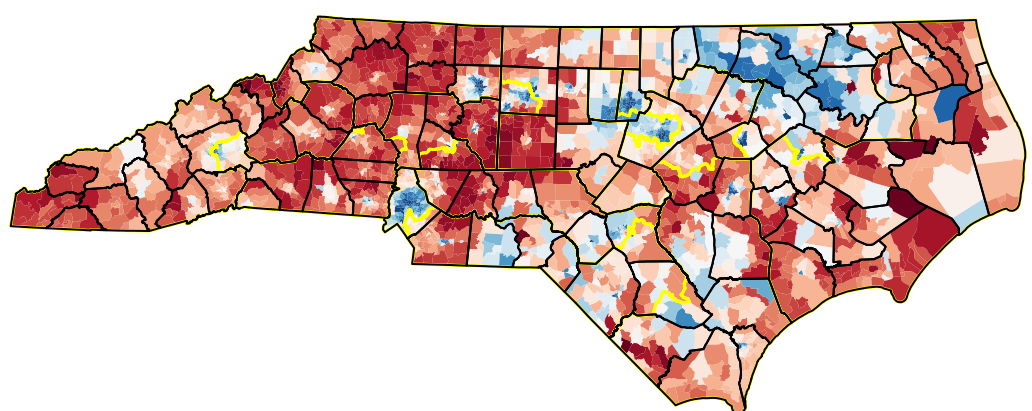
\includegraphics[width=\textwidth]{figs/NC_counties.png}
\caption{North Carolina enacted districts deviation from county boundaries}
\end{figure}
One may observe that where the districts deviate from county boundaries, it is often seemingly to either crack or pack a blue region of precincts -- one may even be tempted to say that ``the gerrymandering happens in the interior of the counties''. We stress that this is just a preliminary analysis, and more study is required.

\item \textbf{Communities-of-interest} -- in some cases, counties represent a community which should be kept whole for the purposes of representing the interests of that community. 

\item \textbf{Election administration} -- to the extent that counties are involved in administering elections, fewer districts means fewer ballots to manage.

\item \textbf{Nested government} -- a general principle of governance is that the various jurisdictions at each level of government be nested.
\end{enumerate}
 
\section{Splitting scores}
It is not always clear what should be meant by ``splitting counties less''. Since it is not always feasible to find even one map that never splits a county (some counties are for example far more populous than any district), trade-offs must be made. In order to compare different plans against one another, one can come up with a score which reflects the extent to which county splitting occurs in the plan. The main body of work in the VRDI project was to propose and analyse a number of different such scores. Here we present some of the more promising scores considered. Again, we consider the case of counties, though other localities can also be considered. In each case, we list what we consider the advantages and disadvantages of the score, as well as any other properties the score has whose value is unclear.

\subsection{Splits}
\textbf{Definition: } The number of counties which intersect more than one district.

\textbf{Advantages:} Perhaps the simplest score, it is easy to explain and to capture in law.

\textbf{Disadvantages:} Is insensitive to geography and splitting counties into more than two, and does not take into account the nature of the split.

\textbf{Other: } All counties treated equally, regardless of population.


\subsection{Pieces}
\textbf{Definition: } For every county $C$ and every district $D$, let $n(C,D)$ be the number of connected components of the intersection $C \cap D$. Then
$$
\text{pieces } = \sum_{C, D} n(C,D).
$$ 
Informally, lay the county and district borders on top of one another and count the number of resulting regions.

\textbf{Advantages:} A fairly simple score to explain, and is sensitive to additional splittings beyond the first. The intersection of a county and district containing more than one connected component often fails the ``eyeball'' test.

\textbf{Disadvantages:} Is insensitive to geography, and does not take into account the nature of the split.

\textbf{Other: } All counties treated equally, regardless of population. Is inherently symmetric in counties and districts.


\subsection{Parts}
\textbf{Definition: } For every county $C$, let $s(C)$ be the number of districts intersecting $C$. Then
$$
\text{parts } = \sum_{C} s(C).
$$ 

\textbf{Advantages:} A fairly simple score to explain, and is sensitive to additional splittings beyond the first. 

\textbf{Disadvantages:} Is insensitive to geography, and does not take into account the nature of the split.

\textbf{Other: } All counties treated equally, regardless of population. Symmetric, as the following lemma shows.

\begin{Lemma}
For every district, let $s(D)$ be the number of counties intersecting $D$. Then
$$
\sum_{C \in \cou} s(C) = \sum_{D \in \dis} s(D)
$$
\end{Lemma}
\begin{proof}
Both sides are merely the number of non-empty sets in the collection
$$
\{ C \cap D \mid C \in \cou,\ D \in \dis \}
$$
\end{proof}

\subsection{Shannon Entropy}
\textbf{Definition: } An information-theoretical concept which asks: on average, how many additional bits of information are required to specify a person's district once the county is known? It is defined by the formula: 
$$
\textsf{ShEnt} = \sum_{C \in \cou} \frac{\pop(C)}{T} \sum_{D \in \dis} - \frac{\pop(C \cap D)}{C} \log \frac{\pop(C \cap D)}{C}
$$
where $T$ is the total population of the state. Note: another variant of this formula considers \emph{number of VTDs} instead of population. 

\textbf{Advantages: } Takes into account the nature of the split. In particular, a $50-50$ split of a county is worse than a $99-1$ split. This may or may not be considered an advantage depending on user preference. Also takes into account county populations.

\textbf{Disadvantages: } Does not consider geography. The score is unitless, and does not make sense to compare across states. It is also not easy to explain to non-experts.

\textbf{Other : } Counties are not treated equally, and are weighted by population.

\subsection{Symmetric square-root entropy}
\textbf{Definition: } A symmetrization of Shannon entropy, replacing $\log$ by square root.

$$
\textsf{SqEnt} = \sum_{C \in \cou} \pop(C) \sum_{D \in \dis} \sqrt{\frac{\pop(C \cap D)}{C}} + 
\sum_{D \in \cou} \pop(D) \sum_{C \in \cou} \sqrt{\frac{\pop(C \cap D)}{D}}
$$
This score was recommended in a footnote of the \emph{Virginia criteria paper}.

\textbf{Advantages: } Takes into account the nature of the split. In particular, a $50-50$ split of a county is worse than a $99-1$ split. This may or may not be considered an advantage depending on user preference. Also takes into account county populations. The symmetry may be appealing in situations where counties differ widely in population relative to an ideal district size.

\textbf{Disadvantages: } Does not consider geography. The score is unitless, and does not make sense to compare across states. It is also not easy to explain to non-experts.

\textbf{Other : } Counties are not treated equally, and are weighted by population.

\subsection{Power entropy}
\textbf{Definition: } This score is based on Shannon entropy, but adapted to penalize small splits more, and to weight low population counties more than high population ones (this apparently inspired by Iowa's recommendation that ``[w]hen there is a choice between dividing local political subdivisions, the more populous subdivisions shall be divided before the less populous''). It is given by the formula

$$
\textsf{PEnt} = \sum_{C \in \cou} \frac{T}{\pop(C)} \left[ \left( \sum_{D \in \dis} \left( \frac{\pop(C \cap D)}{\pop(C)} \right)^{1-\alpha} \right) - 1 \right]
$$
where $\alpha$ is some parameter between $0$ and $1$. We refer the reader to the VRDI 2018 report \emph{Entropy Functions for Analysis of Splittings in Redistricting} for full motivation of this score, where $\alpha = 0.8$ is recommended. Note: as with Shannon entropy, there is a variant using number of VTDs instead of population.

\textbf{Advantages: } Takes into account the nature of the split. In particular, a $50-50$ split of a county is worse than a $99-1$ split. This may or may not be considered an advantage depending on user preference. It penalizes a $99-1$ split and additional small splits more heavily than Shannon entropy does. Also takes into account county populations, though in the opposite sense of Shannon entropy.

\textbf{Disadvantages: } Does not consider geography. The score is unitless, and does not make sense to compare across states. It is also not easy to explain to non-experts. Compared with the Shannon version, it also lacks a historical underpinning from information theory.

\textbf{Other : } Counties are not treated equally, and are \emph{inverse}-weighted by population.


\subsection{Naked boundary}
\textbf{Definition: } The length of district boundary which is not coincident with a county boundary. This ``length'' may be computed either
\begin{enumerate}
\item[{\small$\bullet$}] exactly (in miles), or
\item[{\small$\bullet$}] approximated by the number of cut edges between districts whose ends lie in the same county.
\end{enumerate} 

\textbf{Advantages: } Considers geography, and penalizes ``weird'' intra-county district boundaries which may fail the eyeball test. Simple to explain and in natural units when computed in miles. Appears to line up well with legal language surrounding ``political boundaries''.

\textbf{Disadvantages: } Conflated with compactness in that more compact plans may naturally score lower. Both the miles and cut edges versions have measurement issues (miles may suffer from the coastline effect, while cut edges is sensitive to distribution of units e.g. VTDs). Does not take county population into account. Does not penalize small ``nibbles'' very much.

\textbf{Other: } Not symmetric. 

\textbf{Note: } An early version of this score was called ``coincident boundary''. While the terminology is obsolete, this name appears in some plots below where it should be understood to mean this score.



\subsection{Pennsylvania Fouls}
\textbf{Definition: } Based on legal language from Pennsylvania's redistricting legislation, a county $C$ is considered to a ``Pennsylvania foul'' if it it intersects more than 
$$
P(C) = \lceil \pop(C)/I \rceil+1 
$$
districts, where $I$ is the ideal population of a district. The score is then the total number of Pennsylvania fouls.

\textbf{Advantages: } Depends on the state and county layout, and so attempts to be comparable across states. Is not as complicated or opaque as entropy-based scores, but can be ambiguous unless states precisely.

\textbf{Disadvantages: } Is insensitive to geography and splitting counties into more than a certain threshold, and does not take into account the nature of the split. No penalty for splitting every county into two pieces.


\section{Relationships between scores}

\subsection{A note on ensembles}
While neutral ensembles of plans generated from a Markov chain can be effective tools in determining a baseline for various metrics, these ensembles typically split up counties far more than human-made plans, since they are usually blind to these boundaries. Moreover, it is challenging even to bias a MCMC run towards less county splittings, since neither ReCom nor flip are particularly well-suited to proposing plans which split counties less. As a result, care must be taken when using ensemble methods to compare or evaluate these scores.

\subsection{Human-drawn plans in Pennsylvania}
In order to get some feeling for the scores and how they compare on human-drawn plans, we consider eight plans available in the shapefile for Pennsylvania on github.com/mggg-states. The figures below show the various plans, with districts indicated by colored regions and county boundaries displaying in black.


\begin{figure}[h]
\begin{subfigure}{0.475\textwidth}
\centering
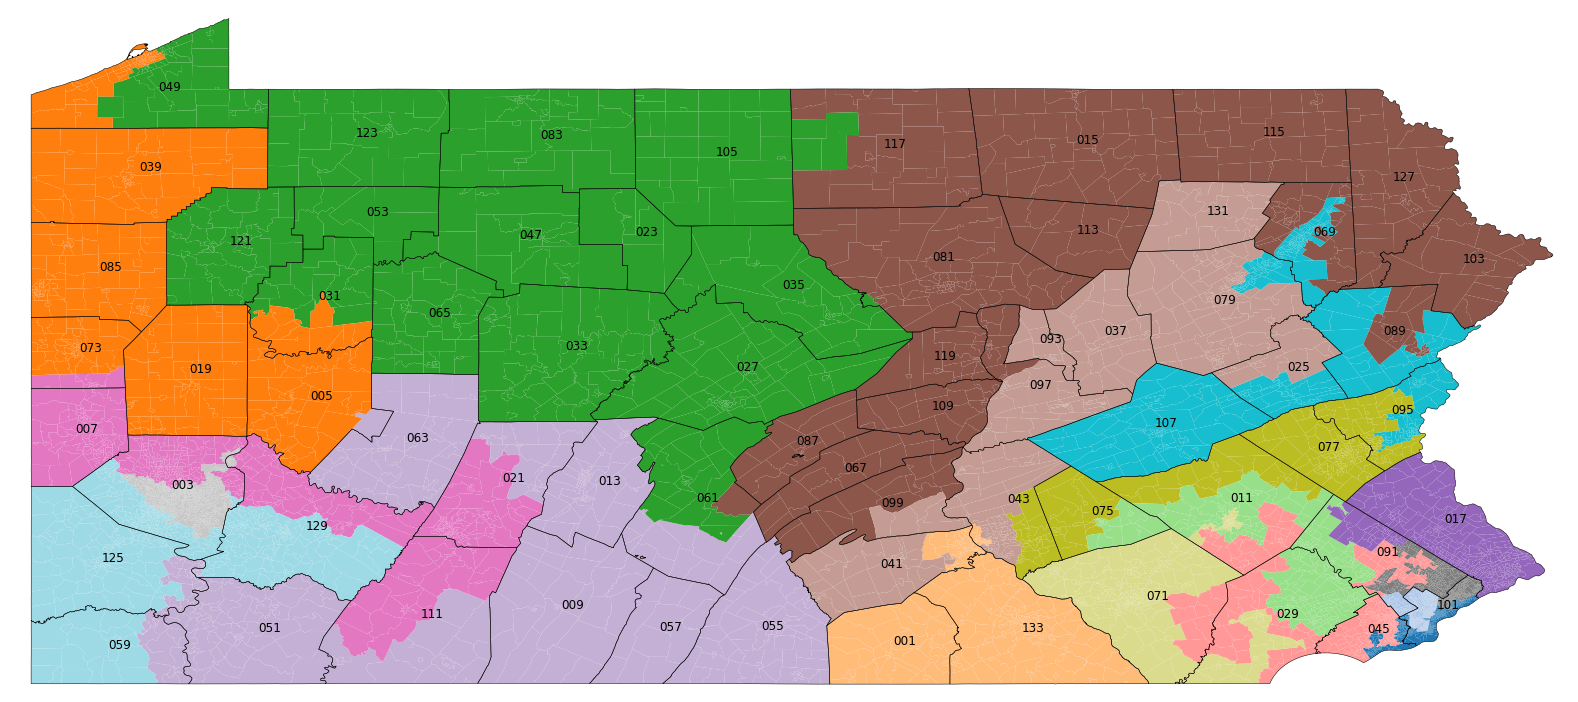
\includegraphics[width=\textwidth]{figs/2011_counties.png}
\caption{2011}
\end{subfigure}
\begin{subfigure}{0.475\textwidth}
\centering
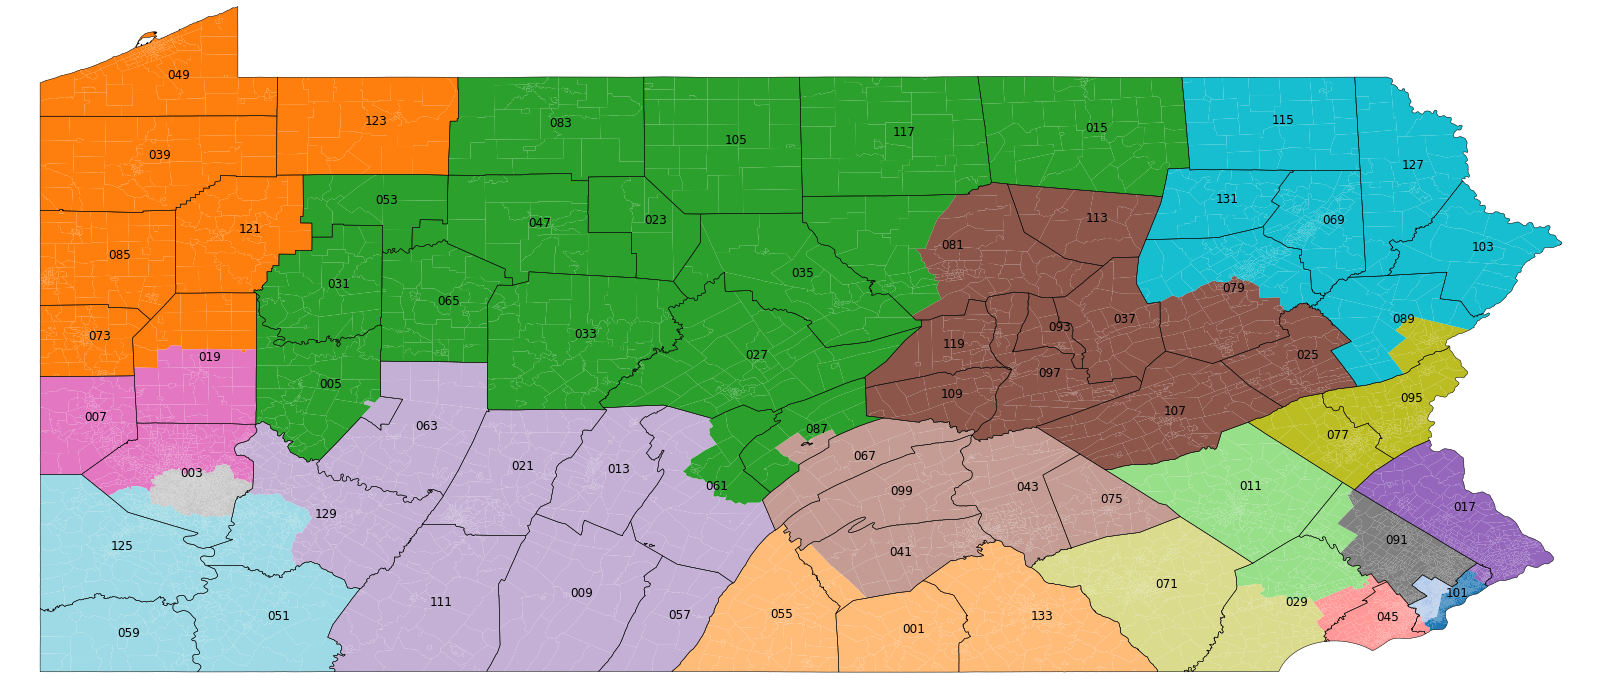
\includegraphics[width=\textwidth]{figs/CPCT_counties.png}
\caption{CPCT}
\end{subfigure}

\begin{subfigure}{0.475\textwidth}
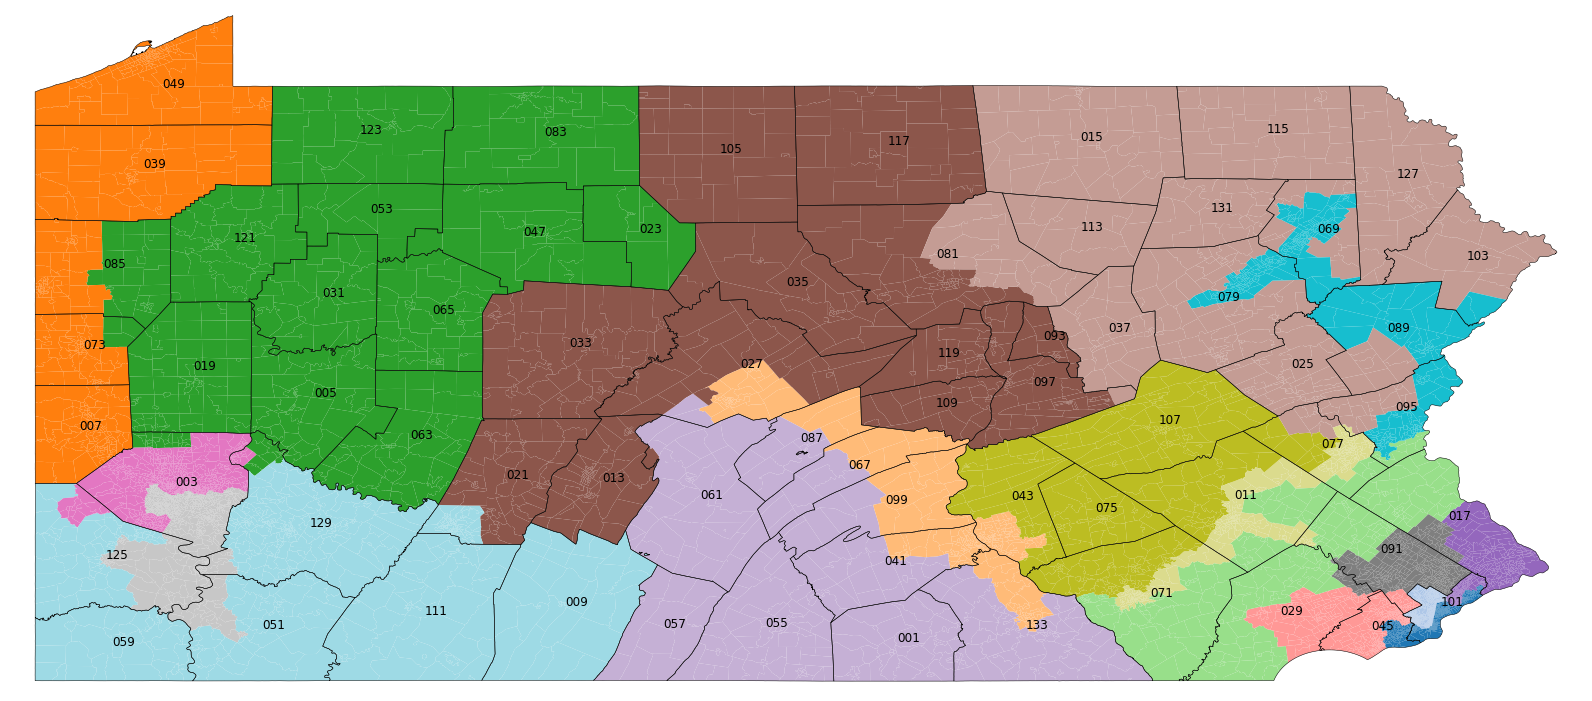
\includegraphics[width=\textwidth]{figs/DEM_counties.png}
\caption{DEM}
\end{subfigure}
\begin{subfigure}{0.475\textwidth}
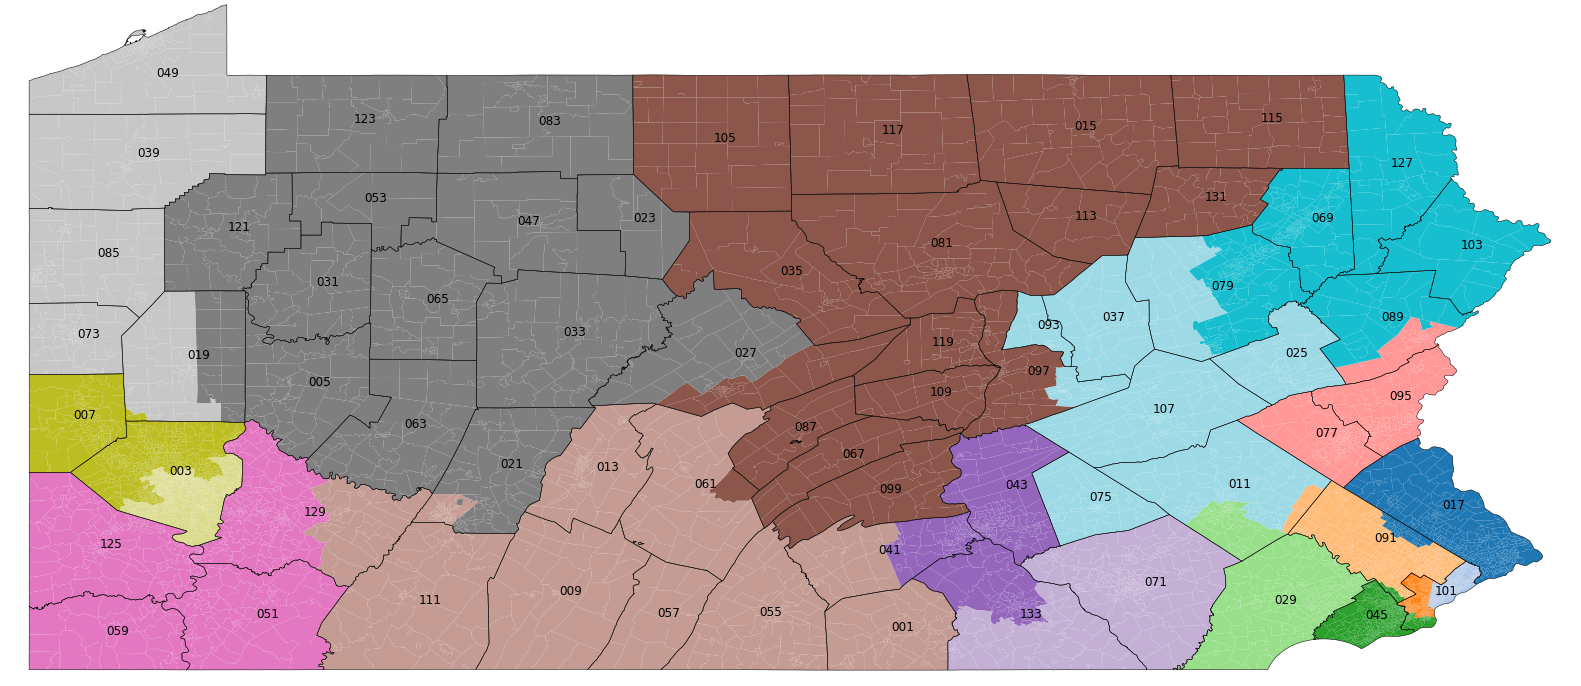
\includegraphics[width=\textwidth]{figs/REMEDIAL_counties.png}
\caption{REMEDIAL}
\end{subfigure}

\begin{subfigure}{0.475\textwidth}
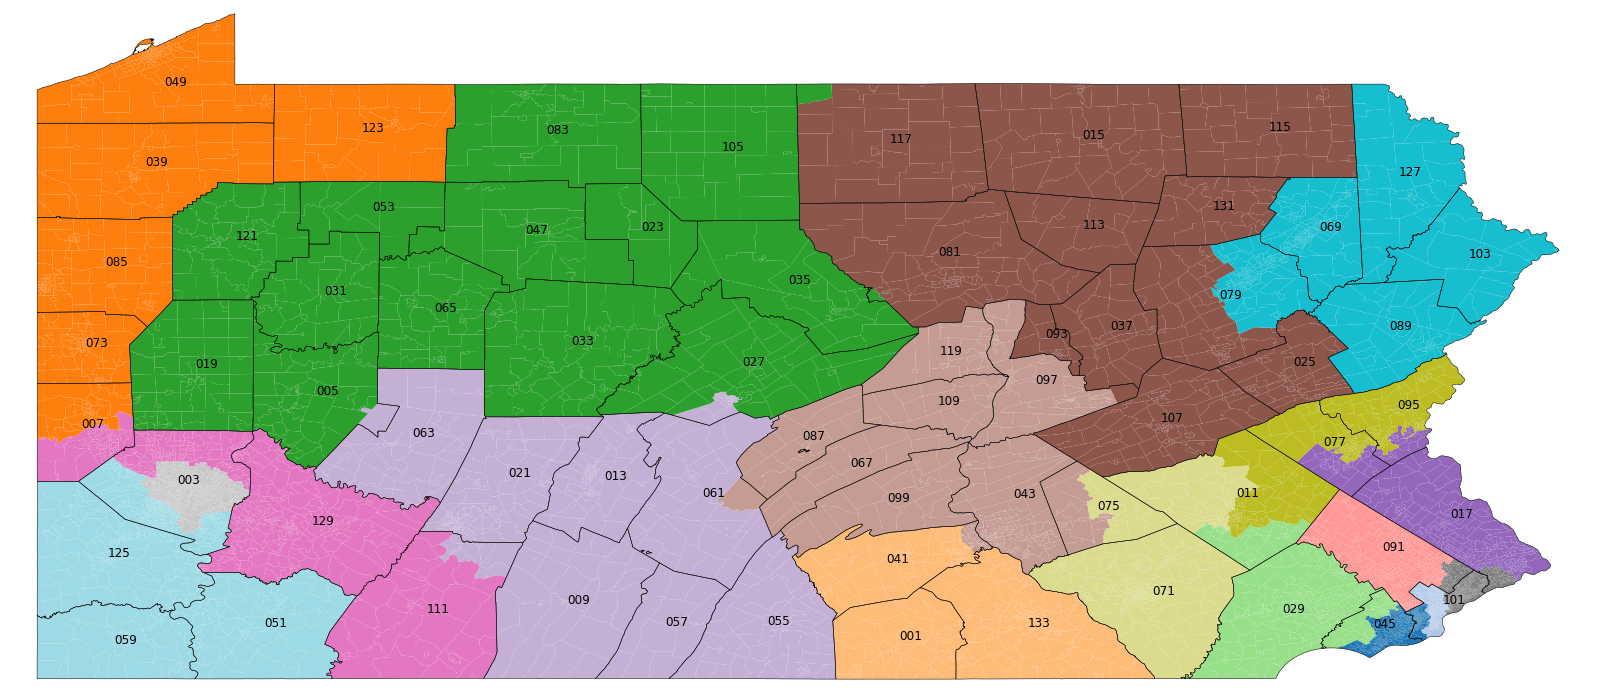
\includegraphics[width=\textwidth]{figs/GOV_counties.png}
\caption{GOV}
\end{subfigure}
\begin{subfigure}{0.475\textwidth}
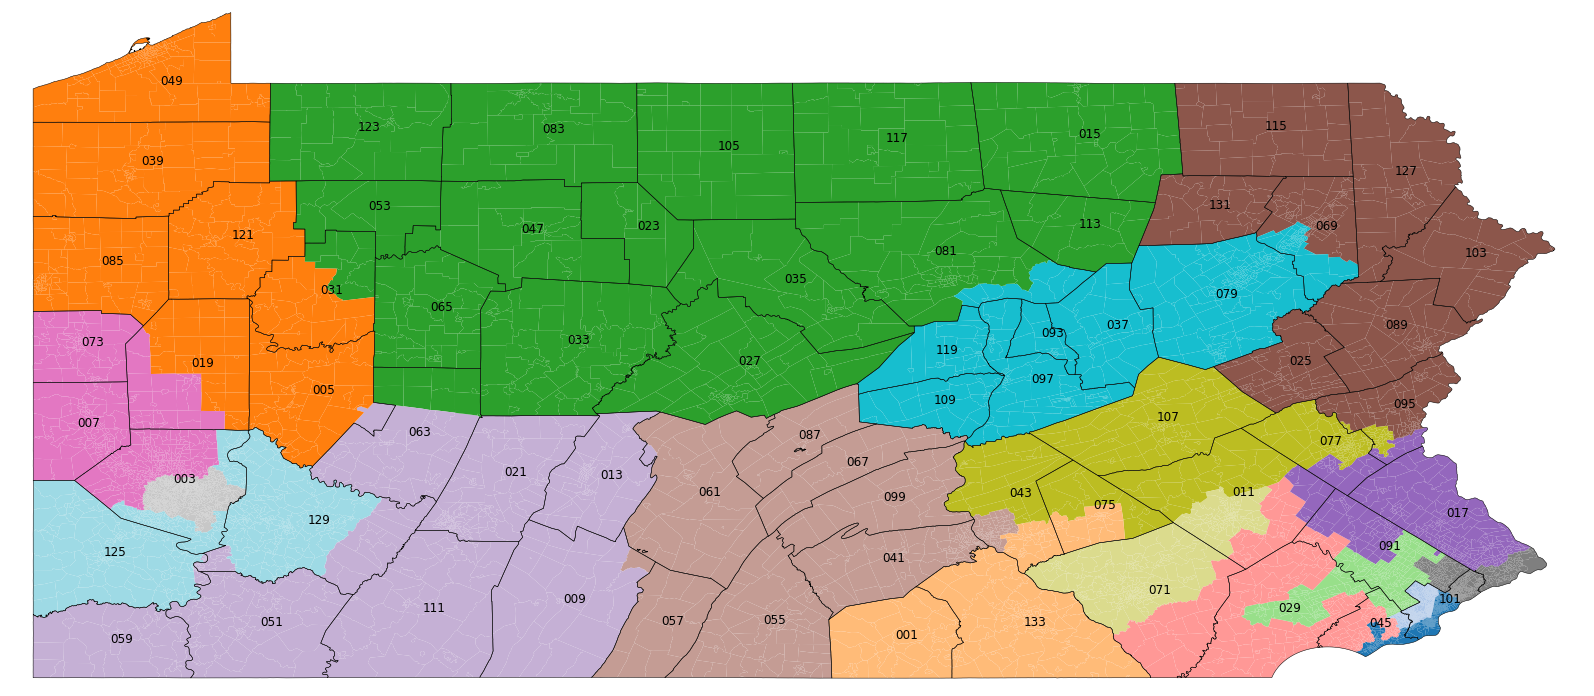
\includegraphics[width=\textwidth]{figs/GOP_counties.png}
\caption{GOP}
\end{subfigure}

\begin{subfigure}{0.475\textwidth}
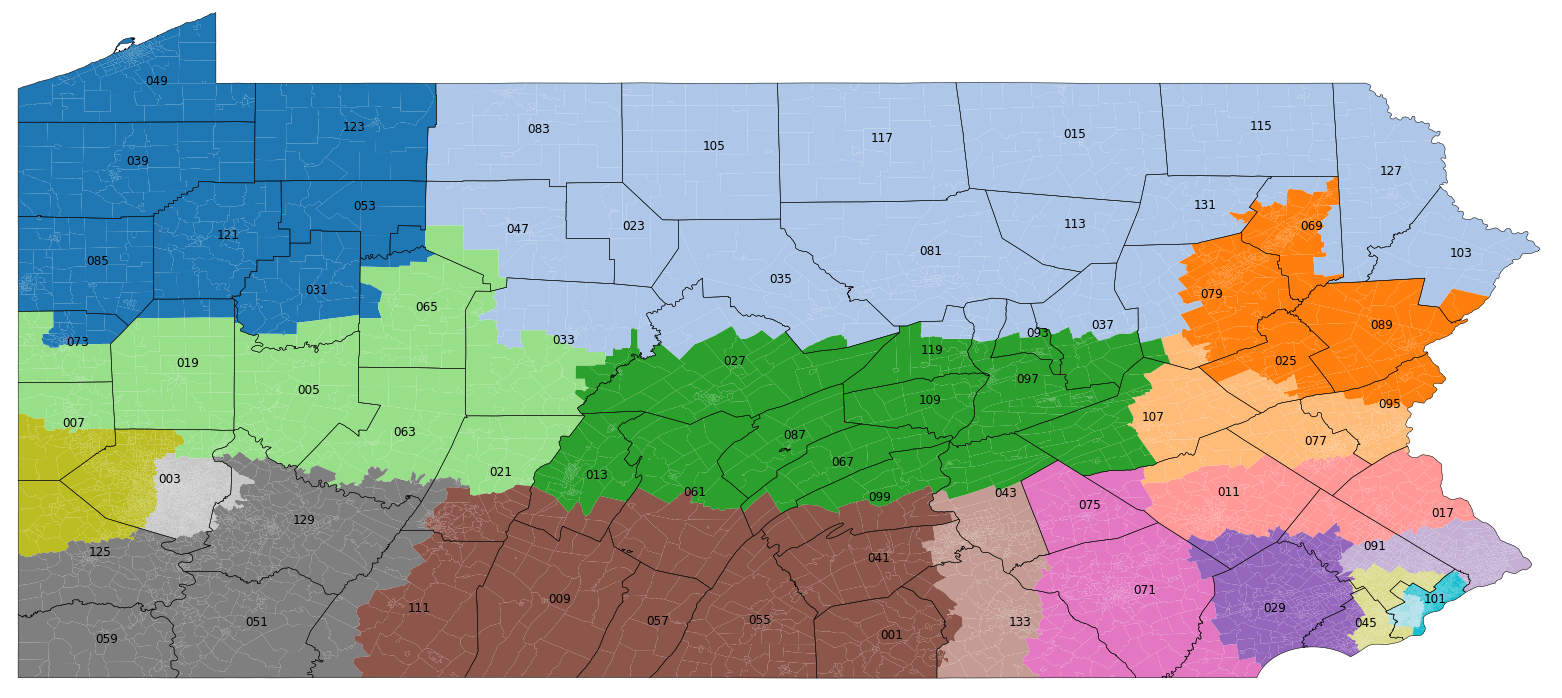
\includegraphics[width=\textwidth]{figs/8th_counties.png}
\caption{8th}
\end{subfigure}
\begin{subfigure}{0.475\textwidth}
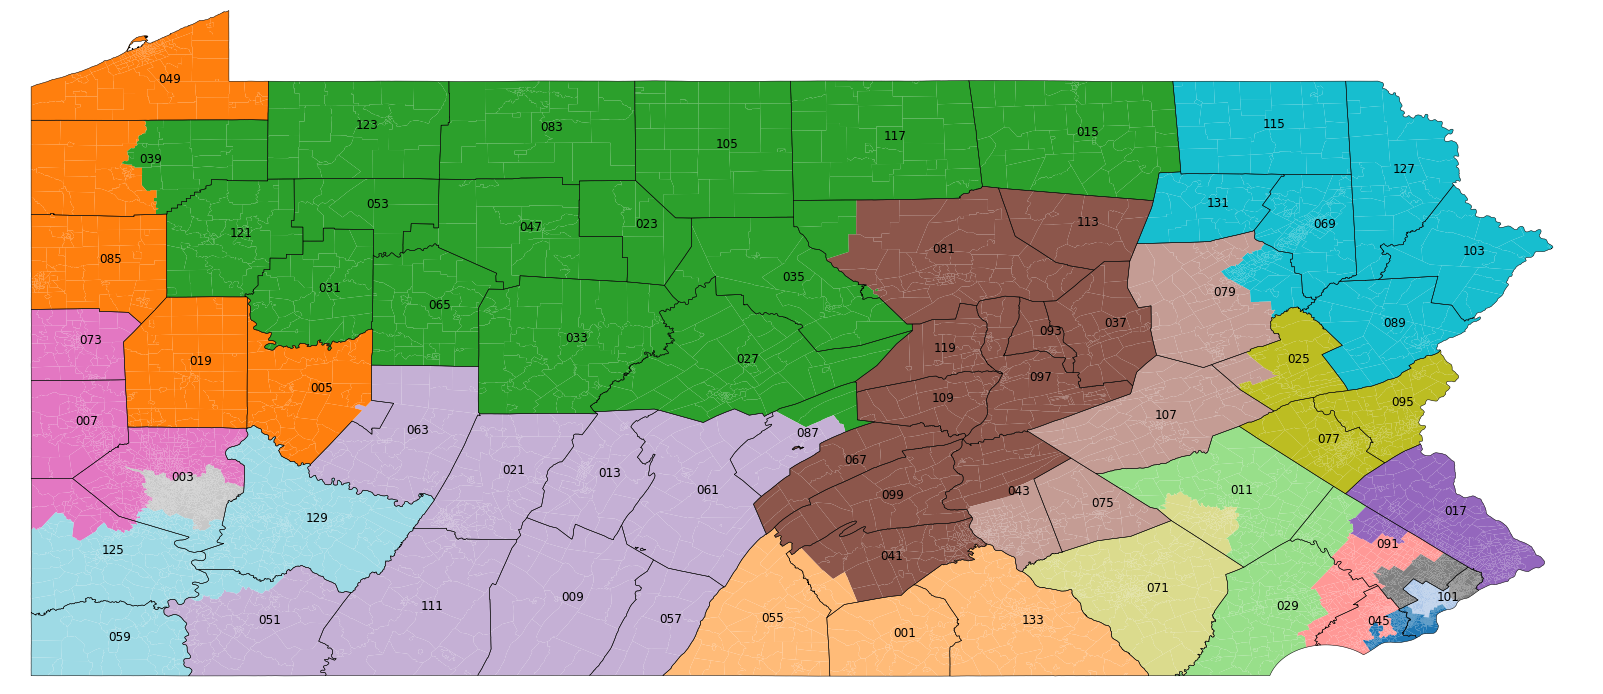
\includegraphics[width=\textwidth]{figs/TS_counties.png}
\caption{TS}
\end{subfigure}

\caption{Human-drawn plans on PA over county boundaries}
\end{figure}

The bar charts below indicate the performance of these eight plans on some of the scores considered above. Note that the VTD variants (not the population variants) of Shannon entropy and Symmetric square-root entropy were used.

Finally, one can compare these scores on the eight plans with scatter plots. While an exhaustive pairwise comparison is possible, for now we restrict to comparing them all against one score (Pieces), which is very simple but also more sensitive than Splits.

\begin{figure}
\centering
\begin{subfigure}{0.4\textwidth}
\centering
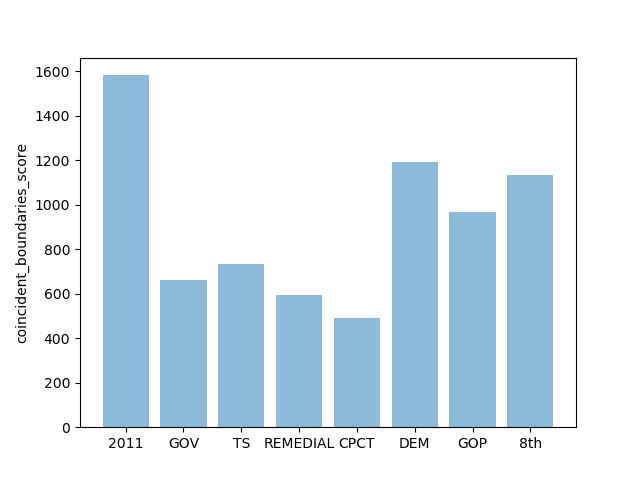
\includegraphics[width=\textwidth]{figs/bars/coincident_boundaries_score_bar.png}
\caption{Naked boundary}
\end{subfigure}
\begin{subfigure}{0.4\textwidth}
\centering
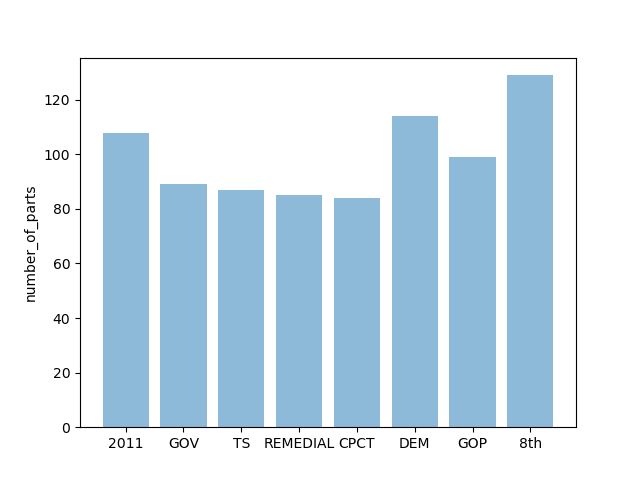
\includegraphics[width=\textwidth]{figs/bars/number_of_parts_bar.png}
\caption{Parts}
\end{subfigure}

\begin{subfigure}{0.4\textwidth}
\centering
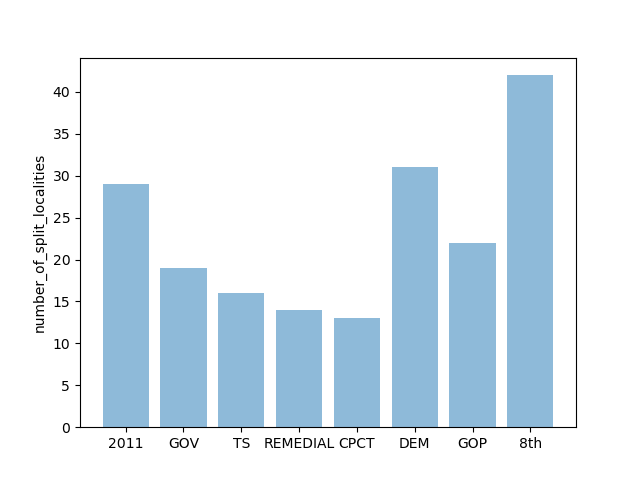
\includegraphics[width=\textwidth]{figs/bars/number_of_split_localities_bar.png}
\caption{Splits}
\end{subfigure}
\begin{subfigure}{0.4\textwidth}
\centering
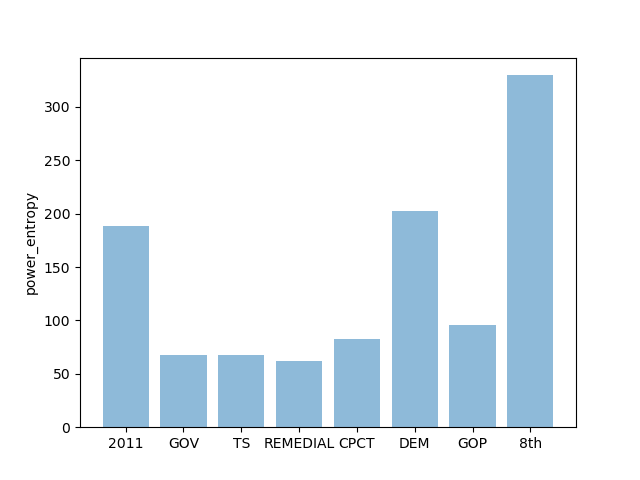
\includegraphics[width=\textwidth]{figs/bars/power_entropy_bar.png}
\caption{Power entropy, $\alpha = 0.8$}
\end{subfigure}

\begin{subfigure}{0.4\textwidth}
\centering
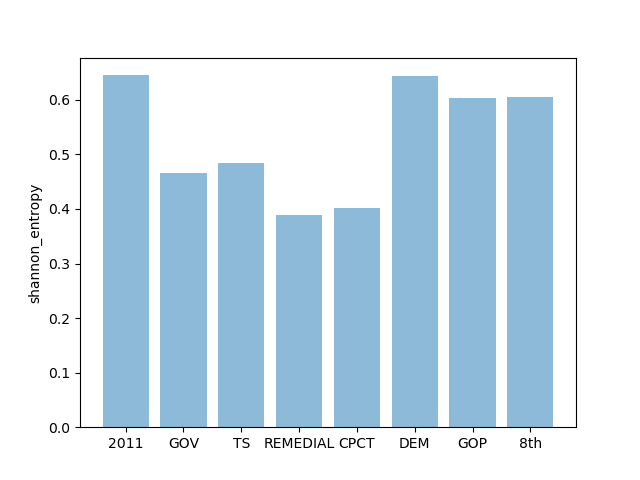
\includegraphics[width=\textwidth]{figs/bars/shannon_entropy_bar.png}
\caption{Shannon entropy}
\end{subfigure}
\begin{subfigure}{0.4\textwidth}
\centering
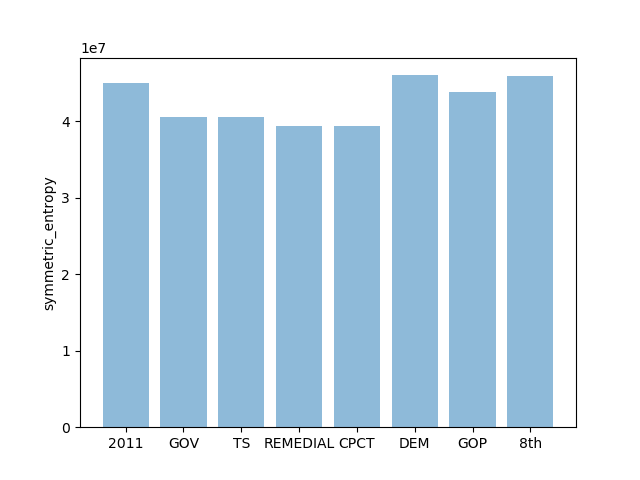
\includegraphics[width=\textwidth]{figs/bars/symmetric_entropy_bar.png}
\caption{Sym. square-root entropy}
\end{subfigure}

\begin{subfigure}{0.4\textwidth}
\centering
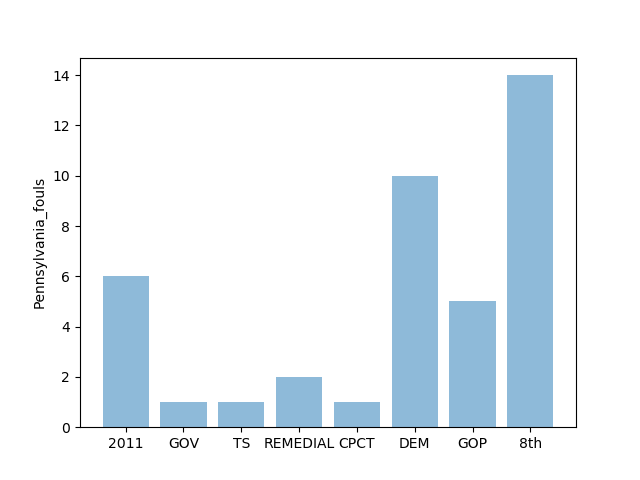
\includegraphics[width=\textwidth]{figs/bars/Pennsylvania_fouls_bar.png}
\caption{Pennsylvania fouls}
\end{subfigure}
\begin{subfigure}{0.4\textwidth}
\centering
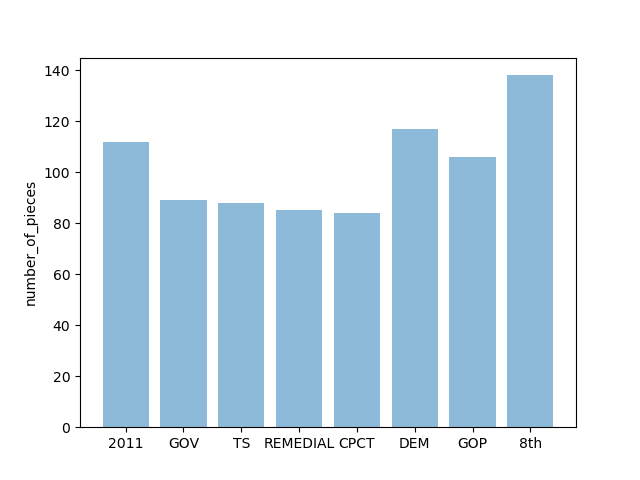
\includegraphics[width=\textwidth]{figs/bars/number_of_pieces_bar.png}
\caption{Pieces}
\end{subfigure}
\caption{Scores for human-drawn plans on PA}
\end{figure}

%%%%%


\begin{figure}
\centering
\begin{subfigure}{0.4\textwidth}
\centering
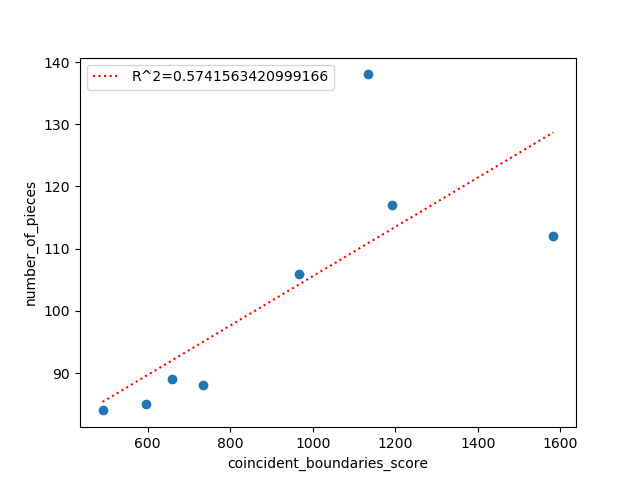
\includegraphics[width=\textwidth]{figs/scatters/cb.png}
\caption{Naked boundary}
\end{subfigure}
\begin{subfigure}{0.4\textwidth}
\centering
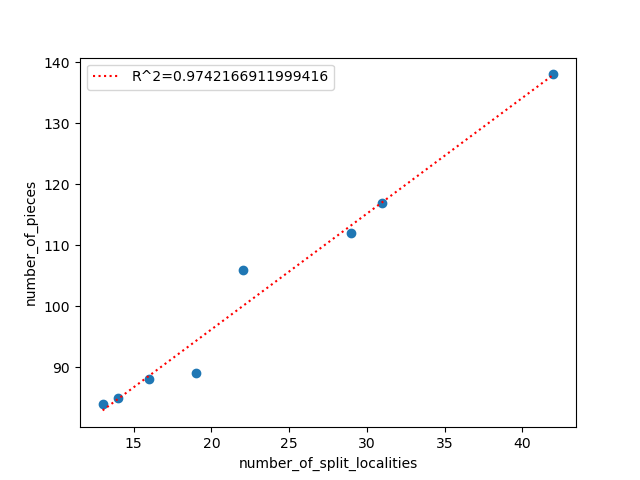
\includegraphics[width=\textwidth]{figs/scatters/splits.png}
\caption{Splits}
\end{subfigure}

\begin{subfigure}{0.4\textwidth}
\centering
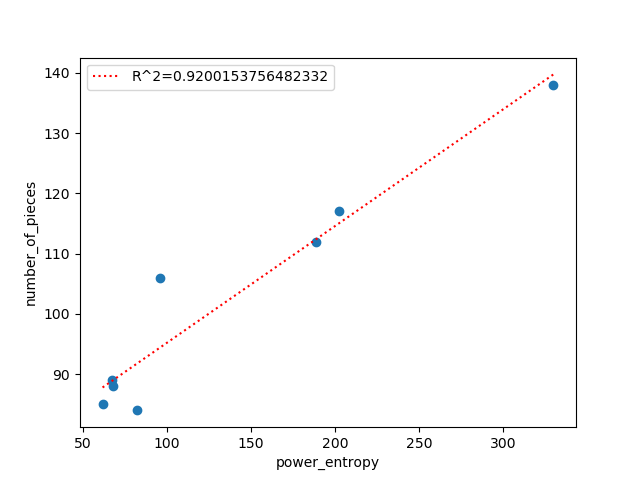
\includegraphics[width=\textwidth]{figs/scatters/pent.png}
\caption{Power entropy, $\alpha = 0.8$}
\end{subfigure}
\begin{subfigure}{0.4\textwidth}
\centering
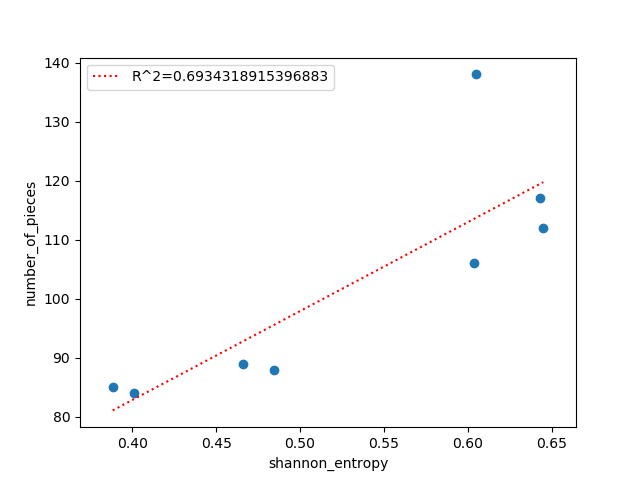
\includegraphics[width=\textwidth]{figs/scatters/shent.png}
\caption{Shannon entropy}
\end{subfigure}

\begin{subfigure}{0.4\textwidth}
\centering
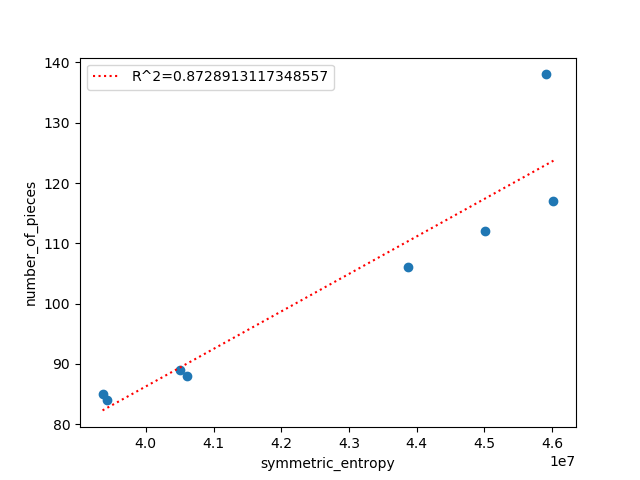
\includegraphics[width=\textwidth]{figs/scatters/syment.png}
\caption{Sym. square-root entropy}
\end{subfigure}
\begin{subfigure}{0.4\textwidth}
\centering
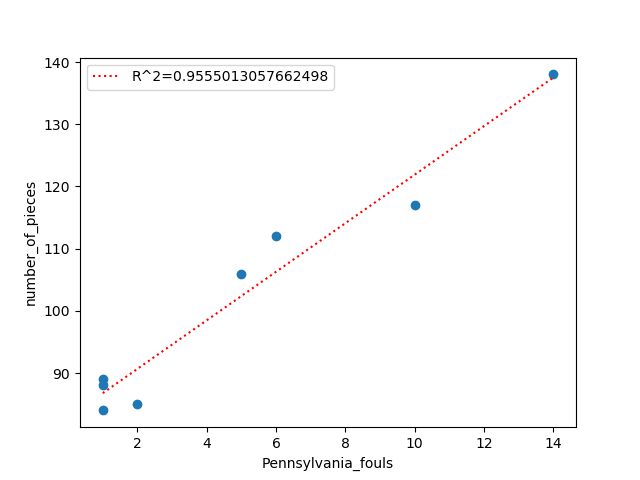
\includegraphics[width=\textwidth]{figs/scatters/Penn.png}
\caption{Pennsylvania fouls}
\end{subfigure}

\begin{subfigure}{0.4\textwidth}
\centering
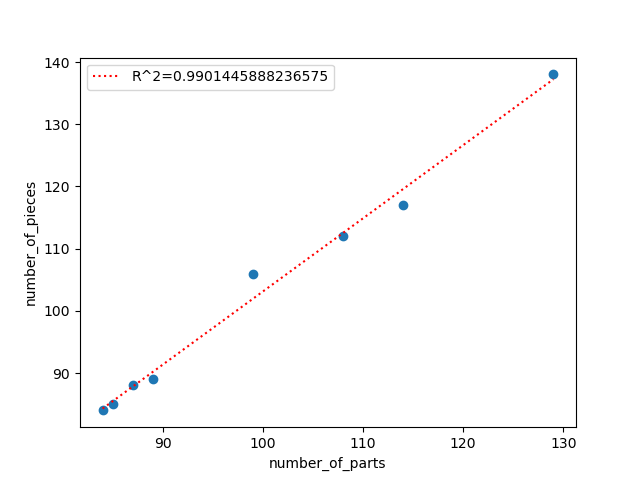
\includegraphics[width=\textwidth]{figs/scatters/parts.png}
\caption{Parts}
\end{subfigure}
\caption{Scatter plots vs Pieces for human-drawn PA plans}
\end{figure}

\subsection{Preliminary short burst ensembles}
We consider using short bursts to optimize for one of these scores and compare how the other scores change. We start these runs from the the remedial PA districting plan and use 500 bursts of 10 steps. We minimize the naked boundary score and compare the other scores on these new districting plans. 

The remedial PA districting plan has 596 cut edges that are not coincident with a county line and this short burst minimization algorithm decreases the number of cut edges to about 460. We find that the naked boundary score is anti-correlated with the number of pieces. In the scatterplot, we have only included the minimum naked boundary districting plan for each short burst.

\begin{figure}[h]
	\begin{subfigure}{0.475\textwidth}
    \centering
    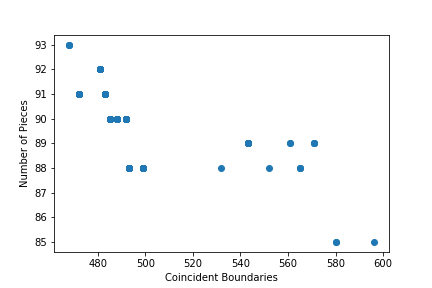
\includegraphics[width=\textwidth]{figs/coin_bound_vs_pieces_5000_10.png}
    \caption{Naked boundary vs. Pieces}
    \end{subfigure}
    	\begin{subfigure}{0.475\textwidth}
\centering
    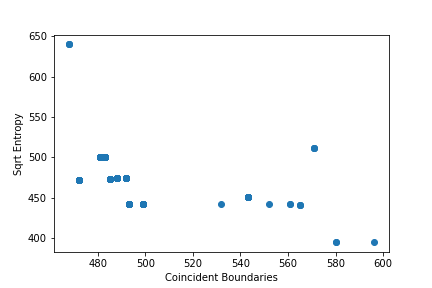
\includegraphics[width=\textwidth]{figs/coin_bound_vs_power_5_entropy_5000_10.png}
    \caption{Naked boundary vs. Sym.}
\end{subfigure}
\caption{Short burst runs on PA}
\end{figure}

We also find that the naked boundary score is anti-correlated with power entropy scores (such as square root entropy and symmetric entropy). However, we find very little correlation with log entropy scores such as Shannon entropy. We can also compare the districting plans of the remedial PA plan and the plan found after 500 short bursts. We find that these plans are quite similar. The minimum naked coincident boundary plan has more splits and pieces than the remedial plan because it takes small nibbles out of counties that add only a few cut edges, but increase the splits and pieces metrics significantly.

\begin{figure}[h]
	\begin{subfigure}{\textwidth}
	        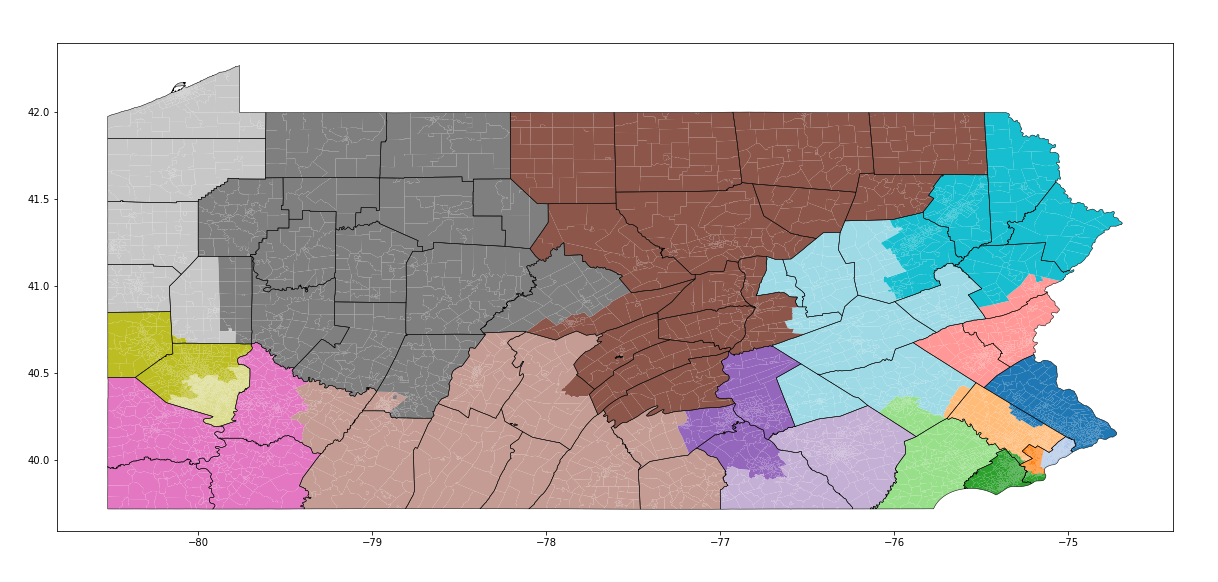
\includegraphics[width=\linewidth]{figs/rem_init_bound.png}
	                 \caption{REMEDIAL plan}
	\end{subfigure}
	
	\begin{subfigure}{\textwidth}
        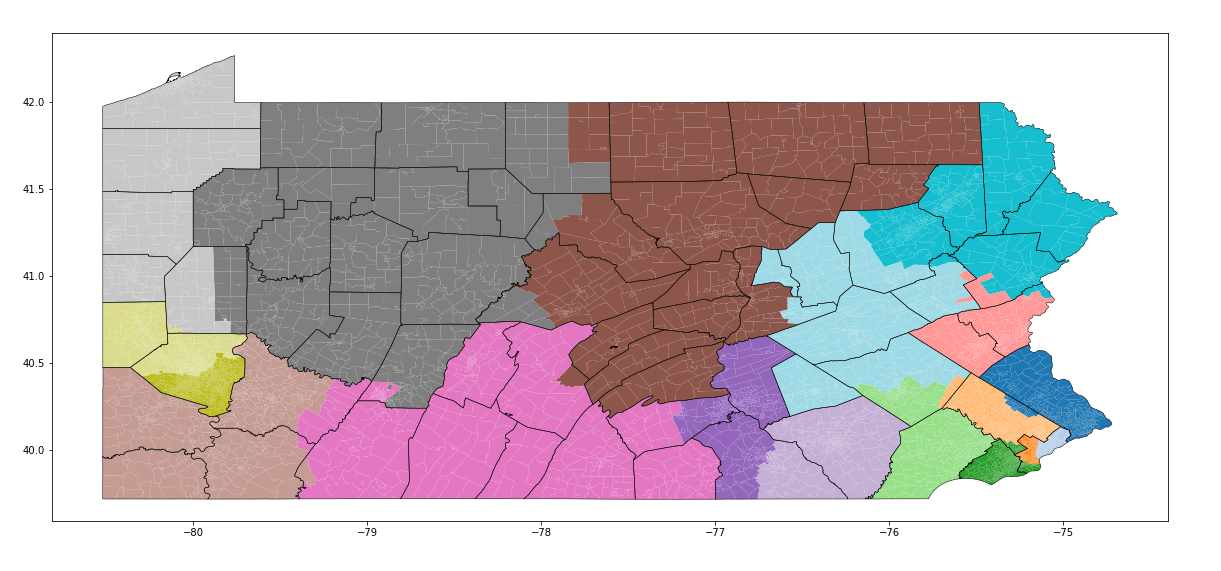
\includegraphics[width=\linewidth]{figs/min_naked_bound.png} 
                 \caption{Min. naked boundary plan}

	\end{subfigure}
     
\end{figure}

A lot more work is needed to design MCMC runs which fully explore plans with similar county splitting properties to human-made plans, to determine if (in this range) these scores are correlated and to what degree. The question of optimizing these scores effectively with MCMC is also the subject of on-going research.



\section{(Tentative) recommendations}
The scores seem to naturally group into three types:
\begin{enumerate}
\item \textbf{Simple counts} -- scores which are easy to understand and compute such as Splits, Parts and Pieces.
\item \textbf{Population-based methods} -- the main characteristic of these scores is they care how the population of a county is divided up (e.g. entropy methods).
\item \textbf{Geography-based methods} -- only Naked boundary represents this class in this report, the main characteristic being that this score cares how the \emph{geography} of a county is divided up.
\end{enumerate}

One can find good reasons to be interested in scores from each of these classes. One should take into account, however, that the simpler scores are easier to codify in law and explain to non-experts. We may tentatively want to recommend that simple counts form the bedrock of questions about county splittings, and thereafter the stakeholders determine for themselves which additional, finer aspects of the problem they care about and whether they are willing to deploy more nuanced and complicated scores.





\end{document}